%================================================================
\chapter{Methodology}\label{chap:methodology}
%================================================================

% Methodology
% Tables with model parameters 
% Sensitivy analysis
% ABC settings, 
% - priors info - noninfo, why?
% - distance 
% - automatic threshold selection
% - reg adjust, loc linear, epkov, why?
% - error measure, RMSPE, SEM

% outline of analysis (perhaps it should be a chapter?)
% - state that we will (try to) identify gbarK & gbarNa, hh model
% - create observed data and extract sumstats, verify the implementations
% - sensitivity analysis
% - focus on hh with abc under different settings (equal n samples)
% - inspect posteriors + ppc
% - test with noisy data -> include eq with current noise
% - SBI on hh 
%
% - Move on to Brunel, eta and g
% - create observation and extract sum stats, verify implementation
% -- since brunelnet is expensive, create only a set for AI state
% - sensitivity analysis
% - ABC
% -- check rmspe vs p-quantile, fixed amount of data
% - posteriors + ppc
% - SBI
% - train on AI and SR state
% - feed one example of each as observation
% - inspect posteriors + ppc

% About MCMC ABC
% MCMC-ABC was also implemented in pyLFI, however, in order to focus the study on the objective, it is not included in the following analyses as it would not give any significant insights into the questions we seek than the more naive rejection sampler would. 
% MCMC methods require a great deal of tuning and diagnosis in order to ensure that the chains actually have converged towards the stationary distribution and sample efficiently (has good mixing).
% The use of MCMC ABC would add an unnecessary layer of complexity to the study.
% Since the focus of this study is not the tuning of the ABC samplers to that extent, we will use the basic rejection sampler for the following analyses. MCMC ABC will not give any other insights that rejction ABC cannot answer for the study at hand 
% However, we decided to include it in such detail because of the revolution MCMC methods brought to Bayesian statistics and that many of the advanced ABC samplers actually build on the MCMC approach. 
% Although rejection and mcmc abc are not the best methods for sampling accurately and efficiently, and scale poorly to higher dimensional problems, they provide a solid basis for understanding more sophisticated/refined sampling schemes and post-hoc adjustments. They showcase that abc provides a robust framework for parameter identification


%================================================================
\section{Outline of Analyses}
%================================================================ 

Here, we provide an outline of the analyses that will be carried out, in order to motivate the following methodologies and give the reader an overview of what is to come. We keep this brief, as we will reiterate the objectives and expand on details as we go along.

The overall objective of this thesis is to investigate the ability and utility of simulation-based inference (SBI) for identifying parameters in mechanistic models of neural dynamics. Specifically, we will investigate the performance of approximate Bayesian computation (ABC) using rejection sampling with post-sampling regression adjustment and the neural density estimation (NDE) algorithm SNPE (see \cref{chap:sbi}). The primary focus will be on ABC, and SNPE will only be used for comparison. 

For the assessment of the strengths and weaknesses of SBI, we mainly use the original Hodgkin-Huxley (HH) model for the potassium (\K), sodium (\Na) and leakage channels found in the squid giant axon membrane (see \cref{sec:hh_model}). The objective of the inferential task on the HH model is to identify the maximum conductance of the \K channel, $\gbarK$, and the maximum conductance of the \Na channel, $\gbarNa$. As such, the remaining parametrization will be kept fixed according to their original values, as tabulated in \autoref{tab:hh_model_parameters}. The observed data will primarily be a synthetically generated voltage trace recording, free of any noise, in order to not have the results overshadowed by noisy data. We will, however, also investigate the impact a noisy recording has on the inference, as real-world neural data are quite noisy. 

Much effort in computational neuroscience today concerns mechanistic models at the network level. We also consider the Brunel network model for activity dynamics in local cortical networks (see \cref{sec:brunel_model}). Here, the inferential task will be to identify the synaptic weight parameters $\eta$ and $g$. The remaining parametrization of the Brunel model will be as given in \autoref{tab:bnet_model_parameters}. For the current study, we primarily limit our analysis to infer the parameters in the asynchronous irregular (AI) state. However, we will try to utilize the flexibility of SNPE by training on simulations from both the AI and synchronous regular (SR) state, to investigate whether the predicted posteriors, when using observed data from one of these states, match the expected parameter ranges from the phase diagram (\autoref{fig:brunel_phase}).

We broadly divide the analyses in two parts, one part concerning the inferential task on the HH model and the other the Brunel network model. In the introduction, we divided the overall objective into six parts:
\begin{enumerate}
    \item Implement simulators for both the Hodgkin-Huxley and Brunel network model in Python. 
    \item Implement a general ABC rejection sampler with post-sampling regression adjustment in Python.
    \item Determine suitable summary statistics of the spiking activity using domain knowledge and develop or find methods for extracting them from the simulated neural data. 
    \item Assess how well the summary statistics constrain the model parameters by examining sensitivity through a correlation analysis. Based on the correlation analysis, implement an importance weighting procedure for the statistics. 
    \item Estimate the model parameter posteriors with both ABC and SNPE by using synthetic observed data generated by the simulators, and examine the performance of the simulation-based inference approach.
    \item Compare the results obtained via ABC and SNPE and insights they might provide about the neuroscientific models. 
\end{enumerate}


%================================================================ 
\section{Summary Statistics of Spiking Activity}
%================================================================ 

The choice of summary statistics is vital in determining the outcome of the inverse modelling with SBI, particularly with ABC algorithms. In the following, we present summary statistics of spiking activity based on domain knowledge.

%================================================================
\subsection{Spike Statistics}\label{sec:spike_statistics}
%================================================================ 

In order to characterize the voltage response of a HH model neuron to depolarizing stimulus, we project the response to low-dimensional summary statistics related to action potential (AP) shape and firing behavior. We will use the spike statistics suggested by Druckmann et al. \cite{druckmann}:

\begin{enumerate}
    \item[(i)] \textbf{Spike rate} -- calculated as the number of spikes divided by the duration of the stimulus;
    \item[(ii)] \textbf{Average AP overshoot} -- calculated by averaging the absolute peak voltage of all APs;
    \item[(iii)] \textbf{Average AP width} -- calculated by averaging the width of every AP at the midpoint between its onset and its peak; 
    \item[(iv)] \textbf{Average AHP depth} -- calculated by averaging all minima voltage throughs, i.e., afterhyperpolarization (AHP) depths, between two consecutive APs;
    \item[(v)] \textbf{Latency to first spike} -- calculated as the time between stimulus onset and first AP peak;
    \item[(vi)] \textbf{Accommodation index} -- calculated as the normalized difference in length of two consecutive interspike intervals (ISIs), i.e., the time between subsequent APs:
    \begin{equation}\label{eq:accomm_index}
        A = \frac{1}{N -k - 1} \sum_{i=k}^N \frac{\mathrm{ISI}_i - \mathrm{ISI}_{i-1}}{\mathrm{ISI}_i + \mathrm{ISI}_{i-1}},
    \end{equation}
    where $N$ is the number of spikes and $k$ determines the number of ISIs that will be disregarded to protect against possible transient behavior. The value for $k = \min \qty(4, N_\mathrm{ISI}/5)$, where $N_\mathrm{ISI}$ is the total number of ISIs. 
\end{enumerate}



%================================================================ 
\subsection{Spike Train Statistics}\label{sec:spiketrain_statistics}
%================================================================ 

From the Brunel network, we record the spike trains from multiple neurons.
Spikes are events characterized by their firing time $t^k$, where $k=1, 2, ...$ labels a spike by the spike count. We define the spike train of a neuron $i$ as the sequence of firing times: 

\begin{equation}
    S_i(t) = \sum_k \delta \left(t - t_i^k \right),
\end{equation}

where $\delta(x)$ is the Dirac $\delta$ function (defined in \cref{sec:recurrent_network}). Thus, spikes are reduced to points in time. In a population of $N$ neurons, we calculate the proportion of active neurons by counting the number of spikes in a small time interval $\Delta t$ and dividing by $N$. Further division by $\Delta t$ yields the population activity:

\begin{equation}
    \nu (t) = \lim_{\Delta t \to 0} \frac{1}{\Delta t} \frac{\int_{t}^{t + \Delta t} \sum_i \sum_k \delta \left(t - t_i^k \right) \dd{t}}{N}
\end{equation} 

In practice, we usually have to bin the spike trains in bins of $\Delta t$ to obtain the time resolved firing rate. 

To characterize the network activity, we will use three summary statistics that aim to capture different aspects of the activity: 
\begin{enumerate}
    \item[(i)] \textbf{Mean firing rate}. We characterize the mean firing rate of the network as a time and population averaged firing rate. This is calculated by first determining the average firing rate of each single spike train by counting its spikes and dividing by a time window, then the population average is found by averaging over all the recorded neurons. 
    \item[(ii)] \textbf{Mean CV}. The regularity of spike trains can be summarized by the spike interval statistic \textit{coefficient of variation} (CV), defined as the standard deviation of the ISIs divided by their mean. The mean CV is calculated by averaging the CV of each neuron's ISIs over all recorded neurons. A regularly spiking neuron would have CV of 0, since there is no variance in the ISIs, whereas a Poisson process has a CV of 1. 
    \item[(iii)] \textbf{Fano factor}. The Fano factor is a statistic across spike trains that measures the variability. It is defined as the variance-to-mean ratio of spike counts in a time window. The Fano factor is typically computed for spike trains representing the activity of the same neuron over different trials. However, since all neurons in the network have identical properties, we can think of the activity of each recorded neuron as a single trial.  
\end{enumerate}


%================================================================
\section{Correlation Analysis \& Importance Weights}\label{sec:corr_analysis}
%================================================================

Some summary statistics may carry more information about a model parameter than others. As the ABC methodology is based on comparing simulated and observed summary statistics, the most informative summary statistics will typically be those with higher variability relative to movement of model parameter values. If we weight the summary statistics in accordance with the variability they exhibit relative to changes in model parameter values, the inferential algorithm might be able to constrain the model parameter better. The notion of weighting the summary statistics in this manner can be said to be a form of \textit{importance weighting}. We would then give larger weights to the summary statistics that are most sensitive to changes in model parameter value and smaller weights to those less sensitive. 

There are numerous robust approaches to base the construction of importance weights on, for instance parameter sensitivity analysis \cite{uncertainpy} or analysis of curvature of an objective function \cite{druckmann}. We will, however, develop a rather simplistic approach where the importance weights are constructed based on correlation analysis. We landed on this approach simply because of the limited time available for carrying out a master project, and this aspect is of lesser importance than others in the study. Nevertheless, the idea behind basing the importance weights on correlation analysis follows. 

Correlation analysis is a method to measure the strength of the linear relationship between the relative movements of two variables $X$ and $Y$. A common measure is the pairwise Pearson's correlation coefficient $r$, which is defined as the ratio between the covariance of the variables and the product of their standard deviations: 

\begin{equation}
    r = \frac{\mathrm{cov}\qty(X, Y)}{\sigma_X \sigma_Y}.
\end{equation} 

As $r$ essentially is a normalized measurement of the covariance, the magnitude of the correlation will be a value between -1 and 1, where the sign indicates the direction of the relationship. A high correlation, i.e., when $r$ is close to 1 or -1, indicates a strong relationship, while $r=0$ points to no relation between the variables.

Correlation analysis, in particular examination of the pairwise Pearson's correlation coefficient matrix, can be used to assess sensitivity by examining which model parameters contribute the most variability to the summary statistics. Thus, correlation analysis may indicate which of the summary statistics might constrain the model parameters the best, though one should keep the assumption of linearity in mind. In practice, assessing the sensitivity via a correlation analysis requires us to perform a pilot study where we sample parameters from the prior predictive distribution, given by \autoref{eq:prior_pred}, and generate the corresponding summary statistics with the simulator model.  

Furthermore, we can use the results from the correlation analysis to construct importance weights for the summary statistics. Given a vector of summary statistics $s = \qty(s_1, ..., s_m)$ and a vector of model parameters $\theta = \qty(\theta_1, ..., \theta_l)$, the following procedure will generate a vector of importance weights $w = \qty(w_1, ..., w_m)$: 
\begin{enumerate}
    \item Given paired samples $\qty{\qty(\theta_k^{(1)}, s_i^{(1)}), ..., \qty(\theta_k^{(n)}, s_i^{(n)})}$ consisting of $n$ pairs where we let $\qty(\theta_k^{(j)}, s_i^{(j)})$ indicate the $j$th sample, we first compute the Pearson correlation coefficient as:
    \begin{equation*}
    r_{i, k} = \frac{\sum_{j=1}^n \qty(\theta_k^{(j)} - \bar{\theta}_k) \qty(s_i^{(j)} - \bar{s}_i)}{\qty[\sum_{j=1}^n \qty(\theta_k^{(j)} - \bar{\theta}_k )^2 \sum_{j=1}^n \qty(s_i^{(j)} - \bar{s}_i )^2 ]^{1/2}},
    \end{equation*}
    where $\bar{\theta}_k$ and $\bar{s}_i$ are the sample means of the $k$th model parameter and the $i$th summary statistic, respectively.
    \item The squared Pearson correlation coefficient, $r_{i,k}^2$, indicates the proportion of variance in $s_{i}$ that is accounted for by (or shared with) $\theta_k$. By definition, $r_{i,k}^2$ will be a number between 0 and 1 that can be used to weight the summary statistics. The summary statistics most sensitive to model parameter movements, will in this way be given a larger weight. Thus, we set the importance weight for $i$th summary statistic for the $k$th model parameter as:
    \begin{equation*}
        w_{i, k} = r_{i, k}^2.
    \end{equation*}
    \item Since the ABC algorithms do not facilitate comparison of summary statistics for individual model parameters, we need to average over all model parameters to obtain the importance weight of the $i$th summary statistic:
    \begin{equation*}
        w_i = \frac{1}{l} \sum_{k=1}^l w_{i, k}.
    \end{equation*}
    \item After obtaining all weights, we ensure that $\sum_{i=1}^m w_i = 1$ by setting each $w_i = w_i / \sum_{i=1}^m w_i$.
\end{enumerate} 




%================================================================
\section{Configuration of ABC Algorithm}
%================================================================ 

Configuring an ABC algorithm for inference requires some choices. In particular, for the rejection ABC algorithm we need to set priors over the model parameters, select a discrepancy metric and a tolerance. In this section we discuss the particular choices we will make. 

%================================================================ 
\subsection{Choice of Priors}
%================================================================ 

In practice, the choice of priors over unknown model parameters is a study in and of itself. Mimicking such a choice is beyond the scope of this thesis. For the present inferential tasks, the choice of priors will regardless be artificial since we actually know the ground truths. For most inferences, we will therefore use noninformative priors to demonstrate the accuracy of the methods based on data alone. For the HH model parameters, we will use priors with about $\pm 10\%$ range around the ground truth parameters. We will, however, also investigate the effect slightly more informative priors have on the convergence of the posterior with the HH model. For the Brunel model, we will only use noninformative priors. For a given observed state, the prior ranges will be set according to the corresponding ranges in the phase diagram of network states (\autoref{fig:brunel_phase}). 

%================================================================
\subsection{Discrepancy Metric}
%================================================================

In ABC algorithms, each simulation is converted to a vector of summary statistics $\ssim = \qty(s_{\mathrm{sim}}^{(1)}, s_{\mathrm{sim}}^{(2)}, ... , s_{\mathrm{sim}}^{(m)})$. We need to define a discrepancy metric that compares each of the simulated statistics in $\ssim$ to the corresponding ones in the vector of observed summary statistics $\sobs$. As discrepancy metric, we will use the Euclidean distance: 

\begin{equation*}
    \rho \qty(\ssim, \sobs ) = \norm{\ssim - \sobs}_2 = \qty[\sum_{i=1}^m \qty(\ssim^{(i)} - \sobs^{(i)} )^2 ]^{1/2}.
\end{equation*}

As illustrated by \autoref{fig:abc_illustration}, the Euclidean distance amounts to a circular acceptance region, which implies identical scales of the summary statistics. However, the summary statistics of spiking activity tend to be on quite different scales, and we will thus be in danger of comparing apples with oranges. The summary statistics with largest scales can dominate any distance calculation unless we normalize the summary statistics so that they vary roughly over the same scale. Scaling the summary statistics in such a manner can be achieved by using a weighted Euclidean distance: 

\begin{equation*}
    \rho \qty(\ssim, \sobs ) = \qty[\sum_{i=1}^m \qty(\frac{\ssim^{(i)} - \sobs^{(i)}}{\sigma^{(i)}} )^2 ]^{1/2},
\end{equation*}

where $\sigma^{(i)}$ is an estimator of the $i$th summary statistic scale. In practice, we need to sample parameters from the prior predictive, feed the parameters to the simulator model and then calculate the empirical scale from the resulting summary statistics. We will scale the summary statistics according to their standard deviation (SD) estimated from the prior predictive samples.  We could have chosen e.g. the median absolute deviation (MAD) as scale instead, which is a more robust estimator of scale than SD. However, if more than 50\% of the prior predictive samples for a particular summary statistic have identical values, MAD will equal zero. We therefore opt for the more reliable SD as scale. 

To extend the above distance metric to include the importance weighting of the summary statistics, the distance metric will be on the form:

\begin{equation}\label{eq:distance_metric}
    \rho \qty(\ssim, \sobs ) = \qty[\sum_{i=1}^m w^{(i)} \qty(\frac{\ssim^{(i)} - \sobs^{(i)}}{\sigma^{(i)}} )^2 ]^{1/2},
\end{equation}

where $w^{(i)}$ is the importance weight of the $i$th summary statistic. If all $w^{(i)}=1$, then the summary statistics are equally weighted. We will use the Euclidean distance on the particular form given by \autoref{eq:distance_metric}. 

%================================================================
\subsection{Semi-Automatic Tolerance Selection}
%================================================================

Determining the tolerance parameter $\epsilon$ in the ABC algorithms can be quite finicky, as we usually do not know in advance exactly what a reasonable cutoff might be. Conceptually, it is easier to require the algorithm to accept some small proportion of the simulations rather than setting $\epsilon$ by hand. If we define the tolerance as the $q$-quantile of the distances from $n$ simulations, we avoid manually setting $\epsilon$. With this quantile-based rejection scheme, defining the tolerance as the 0.5-quantile of the distances amounts to accepting 50\% of the simulations, the 0.3-quantile 30\% of the simulations etc. 

%Requires knowledge about which distances we can expect between simulated and observed summary statistics. We can use the $q$-quantile as a criterion for automatic acceptance threshold selection We define the threshold as the $q$-quantile of the distances from from $N$ samples. pyLFI has procedures for this. We only need to provide the $q$-quantile instead of $\epsilon$. Using the 0.5-quantile amounts to accepting 50\% of the simulations, the 0.3-quantile 30\% of the simulations and so on. 




%================================================================
\section{Performance Metrics}\label{sec:performance_metrics}
%================================================================

Choice of suitable performance metrics are central to any analysis. We discussed methods for summarizing posteriors in \cref{sec:summarize_posterior}. Using KDE (see \cref{sec:kde}) to create a visual representation of obtained posterior samples is a useful first-step, as KDE plots quickly inform us about the shapes and locations of the posteriors. In addition, we should use numerical summaries of the posterior. For each posterior over a model parameter we will both indicate in the KDE plot and provide the value(s) of the MAP estimate and the 95\%-HDI. We will also perform posterior predictive checks (PPCs). 

While all of these summaries enable us to assess the goodness of fit, we will also take advantage of the fact that we have access to the ground truth parameters. Just comparing a point estimate with a ground truth is not a particularly good error measure, since this will not account for the width of the posterior. That is, a wide posterior and a narrow posterior might have nearly identical point estimates close to the ground truth, but the narrow posterior will then clearly be more accurate. We will therefore define an error measure that takes the width of the posterior into account. By definition, there will be more posterior samples in the regions of high density in the KDE representation of the posterior. Thus, by averaging over all the posterior samples, we obtain an implicitly weighted error estimate where the width is accounted for. We will use the \textit{root-mean-square percentage error} (RMSPE) as performance metric, defined as:

\begin{equation}\label{eq:rmspe}
    \mathrm{RMSPE} = \sqrt{\frac{1}{n} \sum_{i=1}^n \qty(\frac{\theta_\mathrm{true}-\hat{\theta}_i}{\theta_\mathrm{true}} )^2} \cdot 100
\end{equation}
where the sum is over all $n$ posterior samples, $\theta_\mathrm{true}$ is the ground truth and $\hat{\theta}_i$ is the $i$th posterior sample. The RMSPE thus evaluates the accuracy of a posterior in terms of the percentage difference between the ground truth parameter and the weighted posterior estimate. 

We aim to investigate different settings of tuning parameters, and will generate several posteriors for the same settings in order to assess variability. In these analyses, we take the RMSPE to be the mean of the RMSPEs of all posteriors for a particular setting. The variability can then be assessed through the \textit{standard error of the mean} (SEM), which is the expected value of the standard deviation of means of several samples. This is estimated from a single sample as:

\begin{equation}\label{eq:sem}
    \mathrm{SEM} = \frac{s}{\sqrt{k}},
\end{equation}

where $s$ is standard deviation of the sample mean and $k$ is the sample size.





%================================================================
%================================================================
%================================================================
%================================================================
%================================================================
%================================================================


%================================================================
\chapter{Computational Approach}\label{chap:comp_approach}
%================================================================ 


%================================================================
\section{Computational Strategies}
%================================================================

In this section, we present an assortment of computational strategies we will use. 


%================================================================
\subsection{Log Densities}
%================================================================

Whenever possible, we compute with logarithmic densities in order to avoid computational overflows and underflows. Exponentiation is performed only when necessary. The Metropolis algorithm (\cref{alg:metropolis}) is an example of where log densities should be used, as it requires evaluation of two densities in the calculation of the ratio. With log densities, the ratio is actually computed as the exponential of the difference of the log densities.   

%================================================================
\subsection{Parameter Transformations}
%================================================================
Before regression adjustment, positive parameters should be log transformed. This will both stabilize the variance of the regression model and make it more homoscedastic. In addition, the log transform guarantees that the adjusted parameter values lie in the range of the prior distribution \cite{ABC_ch3}. The final adjusted values are obtained by exponentiation of the r.h.s. of \autoref{eq:linreg_adj}.


%================================================================
\subsection{Sample from the Prior and Posterior Predictive} 
%================================================================

When we want to do posterior predictive checks, we need to sample from the posterior predictive distribution defined by \autoref{eq:post_pred}. This involves an integral which can be completely avoided by the following iterative two-step process:
\begin{enumerate}
    \item Sample a value of $\theta$ from the posterior $\posterior$. 
    \item Generate a prediction $\hat{y}$ by feeding the value of $\theta$ to:
    \begin{itemize}
        \item[(a)] The likelihood $\lhood$ in the case of likelihood-based inference;
        \item[(b)] The simulator model $\mathrm{M}(\theta)$ in the case of simulation-based inference. 
    \end{itemize}
\end{enumerate}

The result of one iteration will be one sample from the posterior predictive distribution. 

Following a similar logic, we can sample from the prior predictive distribution defined by \autoref{eq:prior_pred} via: 
\begin{enumerate}
    \item Sample a value of $\theta$ from the prior $\prior$. 
    \item Generate a prediction $\hat{y}$ by feeding the value of $\theta$ to:
    \begin{itemize}
        \item[(a)] The likelihood $\lhood$ in the case of likelihood-based inference;
        \item[(b)] The simulator model $\mathrm{M}(\theta)$ in the case of simulation-based inference. 
    \end{itemize}
\end{enumerate}

%================================================================
\subsection{vtrap} 
%================================================================

The HH model contains rate equations that are equivalent to expressions on the form:

\begin{equation*}
    \mathrm{rate} = \frac{x}{\exp \qty(x/y) - 1}.
\end{equation*}

However, such expressions are prone to computational overflow. If $x/y = 0$ or close to zero, then the denominator is zero or really small which leads to infinite or extremely large output. From Taylor series approximation, we can find that the above expression is approximated by:

\begin{equation*}
    \mathrm{rate} = y \qty(1 - \frac{x}{2y})
\end{equation*}

if $x/y << 1$. See \autoref{sec:Appendix B} for the derivation. This expression is similar to how the NEURON simulator \cite{neuron_book} handles indeterminate cases for HH style rate equations, and is called \textit{vtrap} in their software. We will also refer to this approximation as vtrap. The HH model rate equations on this form will thus be computed by:

\begin{equation}\label{eq:vtrap}
    \mathrm{vtrap} = \begin{cases}
    y \qty(1 - \frac{x}{2y}) \qquad &\text{if } \frac{x}{y} << 1
    \\
    \frac{x}{\exp \qty(x/y) - 1} \qquad &\text{otherwise}
    \end{cases}
\end{equation}

%================================================================
\subsection{A More Efficient Metropolis Sampler}
%================================================================

Due to complex simulator models, it is not uncommon for the data generation step in ABC algorithms to be expensive and thereby dominate the computational overheads of the algorithms. In the MCMC ABC algorithm (\cref{alg:mcmcabc}), there is actually no need to run forward the simulator model if the proposal parameter is rejected by the Metropolis acceptance criterion, which typically will be less expensive to evaluate. Therefore, the MCMC ABC algorithm can, in general, be formulated in a more efficient manner by changing the order of the required computations, as shown in \cref{alg:mcmcabc_efficient}. 

\begin{algorithm}[!htb]
\caption{Efficient MCMC ABC with Metropolis sampler}
\label{alg:mcmcabc_efficient}
\SetAlgoLined
\DontPrintSemicolon
 % Algorithm 
 \textbf{Initialize\,:}\;
 \nl Sample $\theta_0$ by performing one iteration of rejection ABC (\cref{alg:rej_abc}).\;

 \vspace{5mm}
 \textbf{Sampling\,:}\;
 \For{$t=1, ..., N$}{ 
 \nl Generate proposal $\theta^* \sim q \qty(\theta^* \mid \theta_{t-1})$. \; 
 \nl Calculate acceptance criterion $\alpha = \min \qty(1, \frac{\pi \qty(\theta^*)}{\pi \qty(\theta_{t-1})})$. \; 
 \nl Sample $u \sim \mathrm{U}(0,1)$. \; 
 \vspace{2mm}
 \eIf{$u \leq \alpha$}{
 \nl Simulate data $\ysim $ from $M \qty(\theta^*)$. \;
 \nl Calculate $\rho \equiv \rho \qty(S \qty(\ysim), S \qty(\yobs)) = \rho \qty(\ssim, \sobs)$. \; 
  \eIf{$\rho \leq \epsilon$}{
  \nl  $\theta_t = \theta^*$\;
  }{
  \nl $\theta_t = \theta_{t-1}$\;
  }
   }{
  \nl $\theta_t = \theta_{t-1}$\;
  }
 }
\end{algorithm}


%================================================================
\subsection{Parallelization}
%================================================================

The ABC algorithms are so-called \textit{embarrassingly parallelizable}, which means there is little to no effort to divide the workload as the computations are independent. We will therefore parallelize the ABC samplers we implement ourselves. In the case of rejection ABC, we sample independent posterior samples. Hence, the prescribed number of posterior samples the sampler has to generate can be fairly divided between all available workers. In the case of MCMC ABC, the posterior samples are not independent due to the dependent Markov chains. Parallelizing a single chain is not a straightforward task, but we could let multiple chains sample independently in parallel. As each chain needs sufficient time to converge towards the stationary distribution, each will need a sufficient number of posterior samples to generate in its workload.

%================================================================
\section{Software Development}\label{sec:software}
%================================================================

As part of the thesis, we developed two Python packages; \cw{pyLFI}\footnote{\url{https://github.com/nicolossus/pylfi}} for the implementation of ABC algorithms and regression adjustment, and \cw{NeuroModels}\footnote{\url{https://github.com/nicolossus/neuromodels}} for the implementation of the neural simulator models and methods for summary statistic extraction. Both packages are available via the Python Package Index (PyPI)\footnote{\url{https://pypi.org}}. Besides personal preference, Python was chosen as programming language for several reasons; it is open source, allows for easy, flexible coding and have a plethora of available packages for analysis and visualizations. Moreover, for heavier computations, many Python packages interface with procedures written in faster languages like C. Most of the code is written using either Python's standard library or the standard scientific libraries \cw{NumPy} \cite{numpy}, \cw{SciPy} \cite{scipy}, \cw{Matplotlib} \cite{matplotlib}, \cw{pandas} \cite{pandas} and \cw{seaborn} \cite{seaborn}. For parallelization we used \cw{Pathos} \cite{pathos}, which is a convenient wrapper of the \cw{multiprocessing} package in the standard library. For implementations regarding the Brunel network model, we used \cw{NEST} \cite{nest}, \cw{Neo} \cite{neo} and \cw{Elephant} \cite{elephant}. In addition, SNPE is implemented by its creators in a Python package called \cw{sbi} \cite{sbi}. 

We will not dive into too much detail regarding the implementation of \cw{pyLFI} and \cw{NeuroModels}, as the code itself is fairly documented and available for those interested. In the following, we instead focus on a broader overview of the implementation and brief demonstrations of usage.

%================================================================
\subsection{NeuroModels}\label{sec:neuromodels}
%================================================================

\cw{NeuroModels} is toolbox for simulating neuroscientific models, post-simulation analysis and feature extraction. Here, we provide some implementation details and examples of usage of the different modules. 

\subsubsection*{HH Solver}

We made a general and flexible solver class of the HH model. The coupled differential equations are solved by using \cw{scipy.integrate.solve_ivp}. The numerical integration method can be selected by the user, but in the present study we use the default explicit Runge-Kutta method of order 5(4) (RK45) \cite{RK45}. \cref{lst:hh_solver} shows an example of usage.


% ---------------------------------------------------------------------
\begin{lstlisting}[language=python, label={lst:hh_solver}, caption={Example usage of the HH solver.}]
import neuromodels as nm

# The simulation parameters needed are the simulation time,
# time step and input stimulus:
T = 50.     # Simulation time [ms]
dt = 0.01   # Time step 

# Stimulus can be provided as either a scalar, array or callable
stimulus = nm.stimulus.Constant(I_amp=10,
                                t_stim_on=10,
                                t_stim_off=40
                                )

# Initialize the Hodgkin-Huxley system; model parameters can either
# be set in the constructor or accessed as class attributes:
hh = nm.solvers.HodgkinHuxleySolver(V_rest=-65)
hh.gbarK = 36.0

# The system is solved by calling the class method `solve`:
hh.solve(stimulus, T, dt, method='RK45')

# The solutions can be accessed as class attributes:
t = hh.t
V = hh.V
n = hh.n
m = hh.m
h = hh.h
\end{lstlisting}
% ---------------------------------------------------------------------

\subsubsection*{HH Simulator}

The HH solver is wrapped into a HH simulator class with a call method that takes the conductance parameters as arguments and returns the simulated data. The simulator class also has methods for post-simulation analysis. \cref{lst:hh_simulator} shows an example of usage.

% ---------------------------------------------------------------------
\begin{lstlisting}[language=python, label={lst:hh_simulator}, caption={Example usage of the HH simulator.}]
import matplotlib.pyplot as plt
import neuromodels as nm

# The simulation parameters needed are the simulation time,
# time step and input stimulus:
T = 50.     # Simulation time [ms]
dt = 0.01   # Time step
stimulus = nm.stimulus.Constant(I_amp=10,
                                t_stim_on=10,
                                t_stim_off=40
                                )

# Initialize the Hodgkin-Huxley simulator; simulation and fixed
# model parameters are passed to the constructor:
hh = nm.models.HodgkinHuxley(stimulus,
                             T,
                             dt,
                             method='RK45',     # integration method
                             pdict={},          # dict of model params
                             solver_options={}  # dict of solver opts
                             )

# Calling the instance solves the HH system for the passed values
# of the active conductances, and the voltage trace is returned:
V, t = hh(gbar_K=36., gbar_Na=120.)

# The simulator class has methods for post-simulation analysis, e.g.:
hh.plot_voltage_trace(with_stim=True)
plt.show()
\end{lstlisting}
% ---------------------------------------------------------------------

\subsubsection*{Spike Statistics}

The output voltage trace from the HH simulator needs to be reduced to a set of low-dimensional summary statistics. We implemented procedures for extracting the summary statistics outlined in \cref{sec:spike_statistics}. The extraction of the summaries are based on using \cw{scipy.signal.find_peaks} for identifying spikes that are above a specified firing threshold and separated by a distance greater than the refractory period. Having found the spike positions, most summary statistics can be derived by clever indexing of the voltage and time arrays. Average AP width is extracted via \cw{scipy.signal.peak_widths}, and average AHP depth by passing the negative voltage array (i.e., the flipped voltage trace) to \cw{scipy.signal.find_peaks}. The spike statistics extractor class has a call method that takes the voltage trace as argument and returns the summary statistics specified in the constructor. \cref{lst:spike_stats} shows an example of usage.
% ---------------------------------------------------------------------
\begin{lstlisting}[language=python, label={lst:spike_stats}, caption={Example usage of spike statistics extraction class.}]
import neuromodels as nm

# The simulation parameters:
T = 50.          # Simulation time [ms]
dt = 0.01        # Time step
t_stim_on = 10   # Stimulus onset
t_stim_off = 40  # Stimulus offset
stimulus = nm.stimulus.Constant(I_amp=10,
                                t_stim_on=t_stim_on,
                                t_stim_off=t_stim_off
                                )

# Initialize the Hodgkin-Huxley simulator:
hh = nm.models.HodgkinHuxley(stimulus, T, dt)

# Call simulator to solve system for passed conductances:
V, t = hh(gbar_K=36., gbar_Na=120.)

# Create a list of summary statistics to extract:
stats = ["average_AP_overshoot",
         "spike_rate",
         "average_AP_width",
         "average_AHP_depth",
         "latency_to_first_spike",
         "accommodation_index"]

# Initialize spike statistics extraction class; stimulus onset
# and offset as well as statistics to extract must be passed
# to the constructor:
sps = nm.statistics.SpikeStats(t_stim_on=t_stim_on,
                               t_stim_off=t_stim_off,
                               stats=stats,
                               threshold=0  # find only spikes above 0 mV
                               )

# The SpikeStats instance is callable; the voltage trace must be
# passed as argument. The extracted summary statistics are returned:
sum_stats = sps(V, t)
\end{lstlisting}
% ---------------------------------------------------------------------

\subsubsection*{Brunel Solver} 

We implemented a flexible solver for the Brunel network model using \cw{NEST} inside a Python class. The output of the network is returned as \cw{neo.SpikeTrain} objects, which in turn are specified as \cw{Quantity} objects; these are essentially arrays (or numbers) with a unit of measurement attached. The solver is parallelized through \cw{NEST}. \cref{lst:bnet_solver} shows an example of usage.

% ---------------------------------------------------------------------
\begin{lstlisting}[language=python, label={lst:bnet_solver}, caption={Example usage of the Brunel network model solver.}]
import neuromodels as nm

# Initialize the Brunel network; the `order` parameter determines
# the number of neurons and connections in the network. Model
# parameters can either be set in the constructor or accessed as
# class attributes:
bnet = nm.solvers.BrunelNetworkSolver(order=2500, J=0.35)
bnet.eta = 2.0
bnet.g = 4.5

# The system is solved by calling the class method `simulate`.
# Simulation parameters have default values, but can also be set:
bnet.simulate(T=1000,       # Simulation time [ms]
              dt=0.1,       # Time step
              N_rec=20,     # Number of neurons to record from
              threads=8,    # Number of threads
              )

# The output of the network is returned as `neo.SpikeTrain` objects.
# Whether to return spike trains from excitatory ('exc', default) or
# inhibitory ('inh') neurons is controlled by the `n_type` keyword:
spiketrains = bnet.spiketrains(n_type="exc")

# The `summary` method gives a simple summary of the simulation:
bnet.summary()
\end{lstlisting}
% ---------------------------------------------------------------------

\subsubsection*{Brunel Simulator} 

The Brunel simulator is similar in construction to the HH simulator. It wraps the Brunel solver class and is callable. The call method takes the synaptic weight parameters $\eta$ and $g$ as arguments. The simulator also has methods for post-simulation analysis. \cref{lst:bnet_simulator} shows an example of usage.
% ---------------------------------------------------------------------
\begin{lstlisting}[language=python, label={lst:bnet_simulator}, caption={Example usage of the Brunel simulator.}]
import matplotlib.pyplot as plt
import neuromodels as nm

# Model parameters
order = 2500    # -> NE=10,000 ; NI=2500 ; N_tot=12,500 ; CE=1000 ; CI=250
epsilon = 0.1   # Connection probability
T = 1000        # Simulation time [ms]
N_rec = 20      # Record output from N_rec neurons
n_type = 'exc'  # Record excitatory spike trains
D = 1.5         # Synaptic delay [ms]
J = 0.1         # Excitatory synapse weight [mV]

# NEST settings
threads = 16        # Number of threads to use in simulation
print_time = False  # Print simulated time or not

# Simulator model class constructor:
bnet = nm.models.BrunelNet(order=order,
                           epsilon=epsilon,
                           T=T,
                           N_rec=N_rec,
                           n_type=n_type,
                           D=D,
                           J=J,
                           threads=threads,
                           print_time=print_time,
                           )

# The call method takes the synaptic weight parameters `eta` and `g`
# as arguments and returns the output spike trains:
spiketrains = bnet(eta=2.0, g=4.5)

# The simulator class has methods for post-simulation analysis, e.g.:
bnet.rasterplot_rates()
plt.show()
\end{lstlisting}
% ---------------------------------------------------------------------


\subsubsection*{Spike Train Statistics}

The output spike trains from the Brunel simulator also need to be reduced to a set of low-dimensional summary statistics. We used \cw{Elephant} to extract the summary statistics outlined in \cref{sec:spiketrain_statistics}. The usage of the spike train statistics extractor class is similar to its counterpart for the HH simulator, as shown in \cref{lst:sts}.
% ---------------------------------------------------------------------
\begin{lstlisting}[language=python, label={lst:sts}, caption={Example usage of the spike train statistics extraction class.}]
import neuromodels as nm
import quantities as pq

# Simulator model class constructor:
bnet = nm.models.BrunelNet(order=2500,
                           epsilon=0.1,
                           T=1000,
                           N_rec=20,
                           n_type='exc',
                           D=1.5,
                           J=0.1,
                           threads=16,
                           )

# Simulator call method:
spiketrains = bnet(eta=2.0, g=4.5)

# Create a list of summary statistics to extract:
stats = ["mean_firing_rate",  # rate estimation
         "mean_cv",           # spike interval statistic
         "fanofactor"         # statistic across spike trains
         ]

# Define start and end time as `Quantity` objects:
t_start = 100. * pq.ms  # Cutoff to avoid transient effects
t_stop = 1000 * pq.ms   # End time

# Initialize spike train statistics extraction class;
# start and end time as well as statistics to extract
# must be passed to the constructor:
sts = nm.statistics.SpikeTrainStats(t_start=t_start,
                                    t_stop=t_stop,
                                    stats=stats
                                    )

# The SpikeTrainStats instance is callable; the spike trains must be
# passed as argument. The extracted summary statistics are returned:
sum_stats = sts(spiketrains)
\end{lstlisting}
% ---------------------------------------------------------------------


%================================================================
\subsection{pyLFI}\label{sec:pylfi}
%================================================================

\cw{pyLFI} is a Python toolbox using likelihood-free inference (LFI) (also known as simulation-based inference) for estimating the posterior distributions over model parameters. We have implemented both rejection ABC (\cref{alg:rej_abc}) and MCMC ABC (\cref{alg:mcmcabc_efficient}), as well as post-sampling regression adjustment. We made the software general and flexible, so that it can accommodate other algorithms as well. The price to pay for the generality and flexibility is that the simulation of data and calculation of summary statistics are left entirely to the user. To perform parameter identification with \cw{pyLFI}, there are generally four inputs that need to be specified:
\begin{enumerate}
    \item A simulator model. The mechanistic model needs to be specified through a simulator model that can generate simulated data $\ysim$ for any parameters $\theta$. 
    \item A summary statistics calculator. The ABC algorithms require the use of low-dimensional summary statistics $s = S(y)$ calculated from the raw data $y$. 
    \item Observed data $\yobs$. This must be on the same form as $\ysim$.
    \item A prior $\prior$ for each unknown parameter that describes the range of possible parameter values. 
\end{enumerate}
For each problem, the objective is to estimate the posterior distribution $\pi \qty(\theta \mid \yobs)$. In general, setting up the inference procedure requires three design choices: 
\begin{enumerate}
    \item A distance metric.
    \item Tuning parameters. The number of tuning parameters depend on which ABC algorithm is being used. The central tuning parameter for all algorithms is the threshold $\epsilon$, for which we introduced the alternative quantile-based approach. For MCMC algorithms, there are additional tuning parameters like proposal density scale, burn-in iterations etc. 
    \item Either a simulation budget, i.e. a prescribed number of simulations to run, or a prescribed number of posterior samples the ABC sampler must obtain. Running the simulator is generally the costliest step of the procedure, and many simulator runs might be needed to accurately produce the posterior.
\end{enumerate}

\subsubsection*{Example Usage}

In the following, we demonstrate \cw{pyLFI} on a toy example. We will infer the mean $\mu$ and standard deviation $\sigma$ of a Gaussian distribution with likelihood $p \qty(\yobs \mid \mu, \sigma) = \mathrm{N} \qty(\mu=163, \sigma=15)$, The observed data are sampled from the likelihood: 

% ---------------------------------------------------------------------
\begin{lstlisting}[language=python]
mu_true = 163
sigma_true = 15
likelihood = scipy.stats.norm(loc=mu_true, scale=sigma_true)
obs_data = likelihood.rvs(size=1000) 
\end{lstlisting}
% ---------------------------------------------------------------------

We assume that the likelihood is unknown, and formulate a model to describe the observed data. The model needs to be implemented as a Python callable, i.e., a function or a call method in a class, that is parametrized by the unknown model parameters we aim to infer, here $\mu$ and $\sigma$: 

% ---------------------------------------------------------------------
\begin{lstlisting}[language=python]
def simulator(mu, sigma, size=1000):
    y_sim = stats.norm(loc=mu, scale=sigma).rvs(size=size)
    return y_sim
\end{lstlisting}
% ---------------------------------------------------------------------

Next, we need to reduce the raw data into low-dimensional summary statistics. The summary statistics calculator also needs to be implemented as a Python callable. The function must return the summary statistics as a Python \cw{list} or \cw{numpy.ndarray}. Here, we take the mean and standard deviation to be summary statistics of the data (these are actually \textit{sufficient} summary statistics): 

% ---------------------------------------------------------------------
\begin{lstlisting}[language=python]
def stat_calc(y):
    sum_stats = [numpy.mean(y), numpy.std(y)]
    return sum_stats
\end{lstlisting}
% ---------------------------------------------------------------------

We then place priors over the unknown model parameters using the \cw{pylfi.Prior} class. The signature of the class constructor is: 

% ---------------------------------------------------------------------
\begin{lstlisting}[language=python]
pylfi.Prior(distr_name, *params, name=None, tex=None, **kwargs)
\end{lstlisting}
% ---------------------------------------------------------------------

Here, \cw{distr_name} is passed as a string that correspond to any distribution from \cw{scipy.stats}. \cw{params} are the parameters of the distribution, typically these would be \cw{shape} parameters or \cw{loc} and \cw{scale} passed as positional arguments. \cw{kwargs} are keyword arguments passed to the \cw{SciPy} distribution methods. The \cw{name} keyword argument is required, and is used by \cw{pyLFI} to keep track of the parameter. The \cw{tex} keyword argument is optional, and can be used to provide the \LaTeX \, typesetting for the parameter name. \cw{pyLFI} includes procedures for automatically plotting priors and posteriors, and will use the \cw{tex} name of the parameter as axis labels if provided. The \cw{name} string is used to access the parameters further down the pipeline and is also used as axis labels if \cw{tex} is not provided. 

In the present example, we define the priors: 

% ---------------------------------------------------------------------
\begin{lstlisting}[language=python]
mu_prior = pylfi.Prior('norm',
                       loc=165,
                       scale=2,
                       name='mu',
                       tex='$\mu$'
                       )

sigma_prior = pylfi.Prior('uniform',
                          loc=12,
                          scale=7,
                          name='sigma',
                          tex='$\sigma$'
                          )

priors = [mu_prior, sigma_prior]
\end{lstlisting}
% ---------------------------------------------------------------------

Note that the priors must be collected in a Python \cw{list}. By providing points $x$ to evaluate the prior pdf at, the \cw{pylfi.Prior} class also lets us visualize the priors: 

% ---------------------------------------------------------------------
\begin{lstlisting}[language=python]
import matplotlib.pyplot as plt
fig, axes = plt.subplots(nrows=1, ncols=2, figsize=(5, 2), tight_layout=True)

x = np.linspace(159, 171, 1000)
mu_prior.plot_prior(x, ax=axes[0])

x = np.linspace(11, 20, 1000)
sigma_prior.plot_prior(x, ax=axes[1])

plt.show()
\end{lstlisting}
% ---------------------------------------------------------------------

\begin{figure}[H]
\begin{center}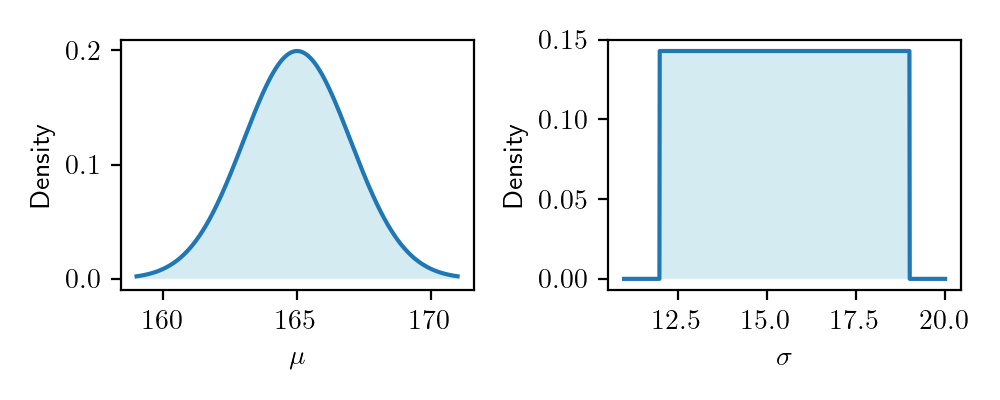
\includegraphics[scale=0.7]{pylfi_prior}
\end{center}
\caption{Priors over $\mu$ and $\sigma$ in the toy example with a Gaussian model.}
%\label{fig:fig1}
\end{figure}

Now, all components needed for inference with \cw{pyLFI} are in place, and we can initialize the ABC sampler: 

% ---------------------------------------------------------------------
\begin{lstlisting}[language=python]
sampler = pylfi.RejABC(obs_data,   # observed data
                       simulator,  # simulator model
                       stat_calc,  # sum stat calculator
                       priors,     # priors over params
                       log=True.   # display logger or not
                       )
\end{lstlisting}
% ---------------------------------------------------------------------

The constructors of the ABC samplers are identical, as each sampler inherit most methods from a general parent class (\cw{pylfi.ABCBase}). 

As mentioned above, there are two approaches for configuring the ABC sampler; we either set a simulation budget or the number of posterior samples to obtain. The latter approach requires a pilot study if we want to estimate $\epsilon$ and the summary statistic scales from the prior predictive distribution. The signature of the pilot study method is: 

% ---------------------------------------------------------------------
\begin{lstlisting}[language=python]
pylfi.ABCBase.pilot_study(nsims,
                          quantile=None, 
                          stat_scale=None,
                          stat_weight=1.,
                          n_jobs=-1,
                          seed=None,
                          )
\end{lstlisting}
% ---------------------------------------------------------------------

The pilot study runs the simulator \cw{nsims} times with parameters sampled from the prior predictive distributions, and sets the tolerance $\epsilon$ automatically as the quantile, specified by the \cw{quantile} keyword, of the simulated distances. If the \cw{stat_scale} keyword is passed as one of the strings \cw{sd} or \cw{mad}, the pilot study also provides an estimate of each summary statistic scales, which are used in the weighted Euclidean distance. \cw{stat_scale='sd'} scales the summary statistics according to their standard deviation (SD) estimated from the prior predictive samples, and \cw{stat_scale='mad'} according to their median absolute deviation (MAD). The \cw{stat_weight} keyword can be used to provide importance weights to the summary statistics. The computational demanding ABC sampler methods are parallelized, and the $\cw{n_jobs}$ keyword can be used to set the number of workers. The default, \cw{n_jobs=-1}, sets the number of workers automatically as the number of found CPUs in the system. Furthermore, the ABC sampler can be seeded via the \cw{seed} keyword. The seed is just provided as an integer. \cw{pyLFI} has procedures for parallel random number generation (PRNG) based on the provided seed, and ensures correct advancement of the underlying PRNG states. This means that the ABC sampler themselves are reproducible, but a caveat of PRNG is that exact reproducibility only is possible when using the same seed and same number of workers. 

For our toy example, performing a pilot study is done as follows: 

% ---------------------------------------------------------------------
\begin{lstlisting}[language=python]
nsims = 1000
sampler.pilot_study(nsims,
                    quantile=0.2,
                    stat_scale="sd",
                    stat_weight=1,
                    n_jobs=4,
                    seed=4
                    )
\end{lstlisting}
% ---------------------------------------------------------------------

To sample from the posterior, we must call the \cw{sample} method, which is specific for each algorithm. For the rejection ABC sampler when a pilot study has been performed, the call becomes: 

% ---------------------------------------------------------------------
\begin{lstlisting}[language=python]
nsamples = 3000
journal = sampler.sample(nsamples,
                         use_pilot=True,
                         n_jobs=4,
                         seed=42,
                         return_journal=True
                         )
\end{lstlisting}
% ---------------------------------------------------------------------

Here, the first positional argument is the number of posterior samples we want. By setting \cw{use_pilot=True}, the sampler will use the tolerance and summary statistic scales found in the pilot study automatically. 
The results of an inference are stored as a \cw{pylfi.Journal} object, which can be returned by setting the \cw{return_journal=True}. The journal can also be accessed through the method:  

% ---------------------------------------------------------------------
\begin{lstlisting}[language=python]
nsamples = 3000
sampler.sample(nsamples,
               use_pilot=True,
               n_jobs=4,
               seed=42
               )
journal = sampler.journal()
\end{lstlisting}
% ---------------------------------------------------------------------

\cw{pylfi.Journal} objects can be both saved to and loaded from disk: 

% ---------------------------------------------------------------------
\begin{lstlisting}[language=python]
# Save journal
filename = 'my_journal.jnl'
journal.save(filename)

# Load journal
journal = pylfi.Journal.load(filename)
\end{lstlisting}
% ---------------------------------------------------------------------

Post-sampling regression adjustment can be performed via a base ABC class method with signature:

% ---------------------------------------------------------------------
\begin{lstlisting}[language=python]
pylfi.ABCBase.reg_adjust(method="loclinear",
                         transform=True,
                         kernel='epkov',
                         return_journal=False
                         )
\end{lstlisting}
% ---------------------------------------------------------------------

The \cw{method} keyword selects the regression method, either linear (\cw{'linear'}) or local linear (\cw{'loclinear'}), the \cw{transform} keyword determines whether or not to take the log transform of the target (the log transform usually gives better regression results) and the \cw{kernel} keyword selects the smoothing kernel, either the Gaussian kernel (\cw{'gaussian'}) or the Epanechnikov kernel (\cw{'epkov'}). 

Thus, performing a local linear regression for our toy example with Epanechnikov kernel and log transform of the the target is coded as: 

% ---------------------------------------------------------------------
\begin{lstlisting}[language=python]
journal = sampler.reg_adjust(method="loclinear",
                             transform=True,
                             kernel="epkov",
                             return_journal=True
                             )
\end{lstlisting}
% ---------------------------------------------------------------------

The obtained posterior samples can be retrieved as a \cw{pandas.DataFrame} from the \cw{pylfi.Journal} class:

% ---------------------------------------------------------------------
\begin{lstlisting}[language=python]
df = journal.df  # pandas DataFrame with posterior samples
\end{lstlisting}
% ---------------------------------------------------------------------

Furthermore, posteriors can be plotted with the \cw{pylfi.Journal.plot_posterior} method. The first positional argument is required and expects a string with the name of a parameter, corresponding to the \cw{name} keyword argument passed to the \cw{pylfi.Prior} constructor. Other options are \cw{hdi_prob} which can be used to set the probability $(1-\alpha)$ of the HDI, \cw{point_estimate} which point estimate to use, either \cw{'map'}, \cw{'mean'} or \cw{'median'}, and \cw{theta_true} to set the ground truth (if available). If \cw{theta_true} is set, then the RMSPE will also be included in the plot. For our present example: 

% ---------------------------------------------------------------------
\begin{lstlisting}[language=python]
fig, axes = plt.subplots(nrows=1, ncols=2, figsize=(8, 3), tight_layout=True)
journal.plot_posterior('mu',
                       hdi_prob=0.95,
                       point_estimate='map',
                       theta_true=mu_true,
                       ax=axes[0]
                       )

journal.plot_posterior('sigma',
                       hdi_prob=0.95,
                       point_estimate='map',
                       theta_true=sigma_true,
                       ax=axes[1]
                       )

plt.show()
\end{lstlisting}
% ---------------------------------------------------------------------


\begin{figure}[H]
\begin{center}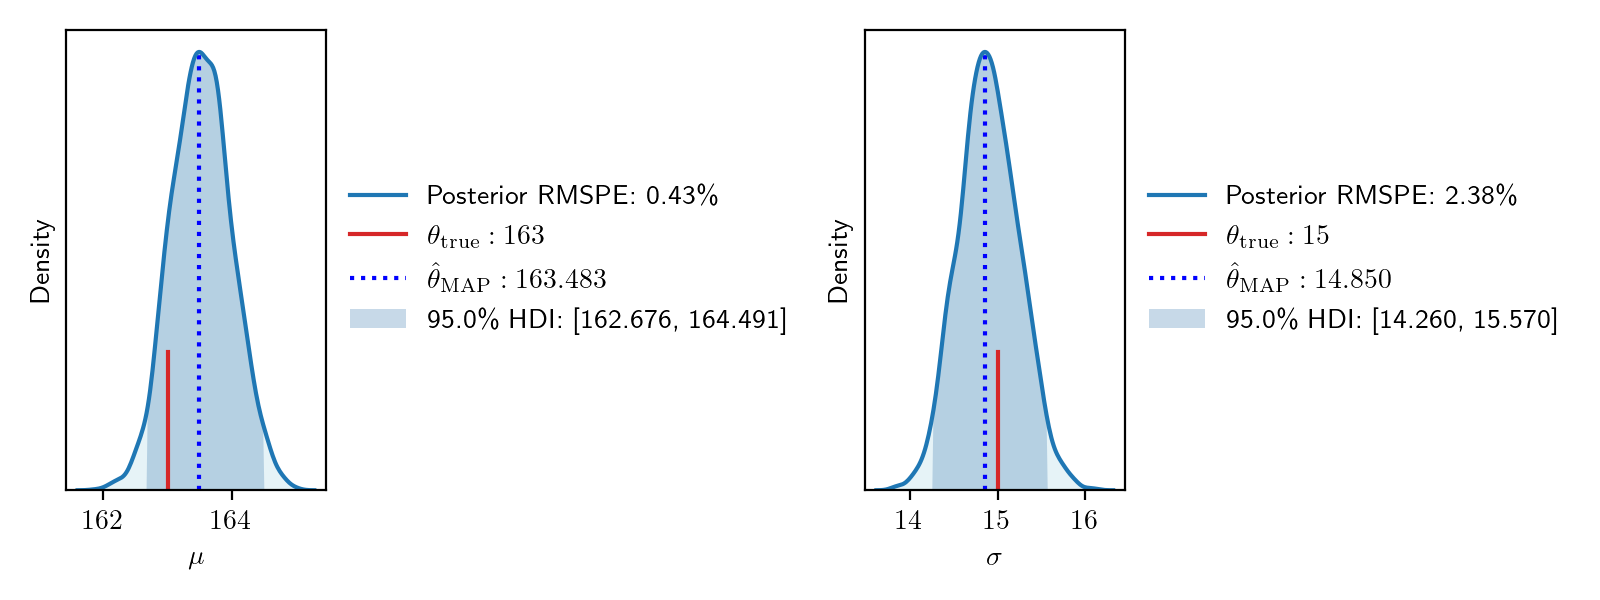
\includegraphics[scale=0.7]{pylfi_posterior}
\end{center}
\caption{Posteriors over $\mu$ and $\sigma$ in the toy example with a Gaussian model.}
%\label{fig:fig1}
\end{figure}


\cref{lst:pylfi} lists a complete script for the usage of \cw{pyLFI} with rejection ABC on the Gaussian toy example: 

% ---------------------------------------------------------------------
\begin{lstlisting}[language=python, label={lst:pylfi}, caption={Example usage of the pyLFI on a Gaussian toy model.}]
import matplotlib.pyplot as plt
import numpy as np
import pylfi
import scipy.stats as stats

# Observed data
mu_true = 163
sigma_true = 15
likelihood = stats.norm(loc=mu_true, scale=sigma_true)
obs_data = likelihood.rvs(size=1000)


# Simulator model
def simulator(mu, sigma, size=1000):
    y_sim = stats.norm(loc=mu, scale=sigma).rvs(size=size)
    return y_sim


# Summary statistics calculator
def stat_calc(y):
    sum_stat = [np.mean(y), np.std(y)]
    return sum_stat


# Priors
mu_prior = pylfi.Prior('norm',
                       loc=165,
                       scale=2,
                       name='mu',
                       tex='$\mu$'
                       )

sigma_prior = pylfi.Prior('uniform',
                          loc=12,
                          scale=7,
                          name='sigma',
                          tex='$\sigma$'
                          )


priors = [mu_prior, sigma_prior]

# Initialize sampler
sampler = pylfi.RejABC(obs_data,
                       simulator,
                       stat_calc,
                       priors,
                       log=True
                       )

# Pilot study
nsims = 1000
sampler.pilot_study(nsims,
                    quantile=0.2,
                    stat_scale="sd",
                    stat_weight=1,
                    n_jobs=4,
                    seed=4
                    )

# Sample posterior
nsamples = 3000
sampler.sample(nsamples,
               use_pilot=True,
               n_jobs=4,
               seed=42
               )

# Local linear regression adjustment
journal = sampler.reg_adjust(method="loclinear",
                             kernel="epkov",
                             transform=True,
                             return_journal=True
                             )


# Plot posteriors
fig, axes = plt.subplots(nrows=1, ncols=2, figsize=(8, 3), tight_layout=True)
journal.plot_posterior('mu',
                       hdi_prob=0.95,
                       point_estimate='map',
                       theta_true=mu_true,
                       ax=axes[0]
                       )

journal.plot_posterior('sigma',
                       hdi_prob=0.95,
                       point_estimate='map',
                       theta_true=sigma_true,
                       ax=axes[1]
                       )

plt.show()
\end{lstlisting}
% ---------------------------------------------------------------------







